\documentclass[tikz, margin=0.25mm]{standalone}

\begin{document}
    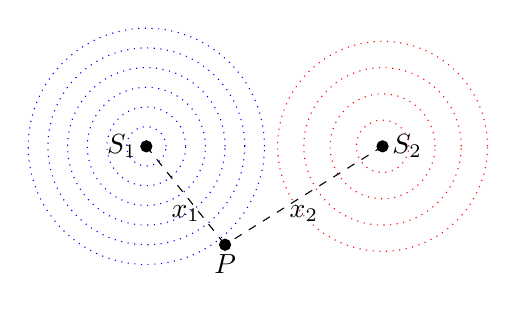
\begin{tikzpicture}
    
    \foreach \ra in {1,...,6}
    \draw[blue,dotted] (0,0) circle (\ra/4);
    
    \foreach \rb in {1,...,4}
    \draw[red, dotted] (3,0) circle (\rb/3);
    
    \filldraw 
    (0,0) circle (2pt) node[left]{$S_1$} 
    (3,0) circle (2pt) node[right]{$S_2$} 
    (1,-1.25) circle (2pt) node[below]{$P$};
    
    \draw[dashed] (0,0) -- node[below]{$x_1$} + (1,-1.25)
    +(3,0) -- node[below]{$x_2$} + (1,-1.25) ; 
        % % axis
        % \draw[->]   (-.25,0) -- + (4.5,0) node[right] {$t$} ;
        % \draw[->] (0,-.25) -- +(0,2) node[above] {$x(t)$};
        % %function
        % \draw[thick, red] plot[domain=0:4*pi, samples=60]  (\x/pi,{sin(\x r)}); 
        % %lambda
        % \draw[dashed]   (1,0) -- + (0,1.4)      (3,0) -- + (0,1.4);
        % \draw[<->]      (1,1.25) -- node[above] {$\lambda$} + (2,0);
        % %amplitude
        % \draw[<->] (0.5,0) -- node[left] {$A$} + (0,-1);
        % \draw[dashed] (.4,-1) -- + (1.375,0);
        % %speed
        % \draw[->] (.25,1.25) -- node[above] {$c$} + (0.5,0);
        % %period
        % \draw[<->] (2,-1.25) -- node[above] {$T$} + (2,0);
        % \draw[dashed] (2,0) -- +(0,-1.4) (4,0) -- +(0,-1.4);
    \end{tikzpicture}  
\end{document}